\setcounter{figure}{3}
\begin{figure}[H]
\centering
\par\smallskip\textbf{Panel 4; current provisional independent calculation: partially reproduced}\par
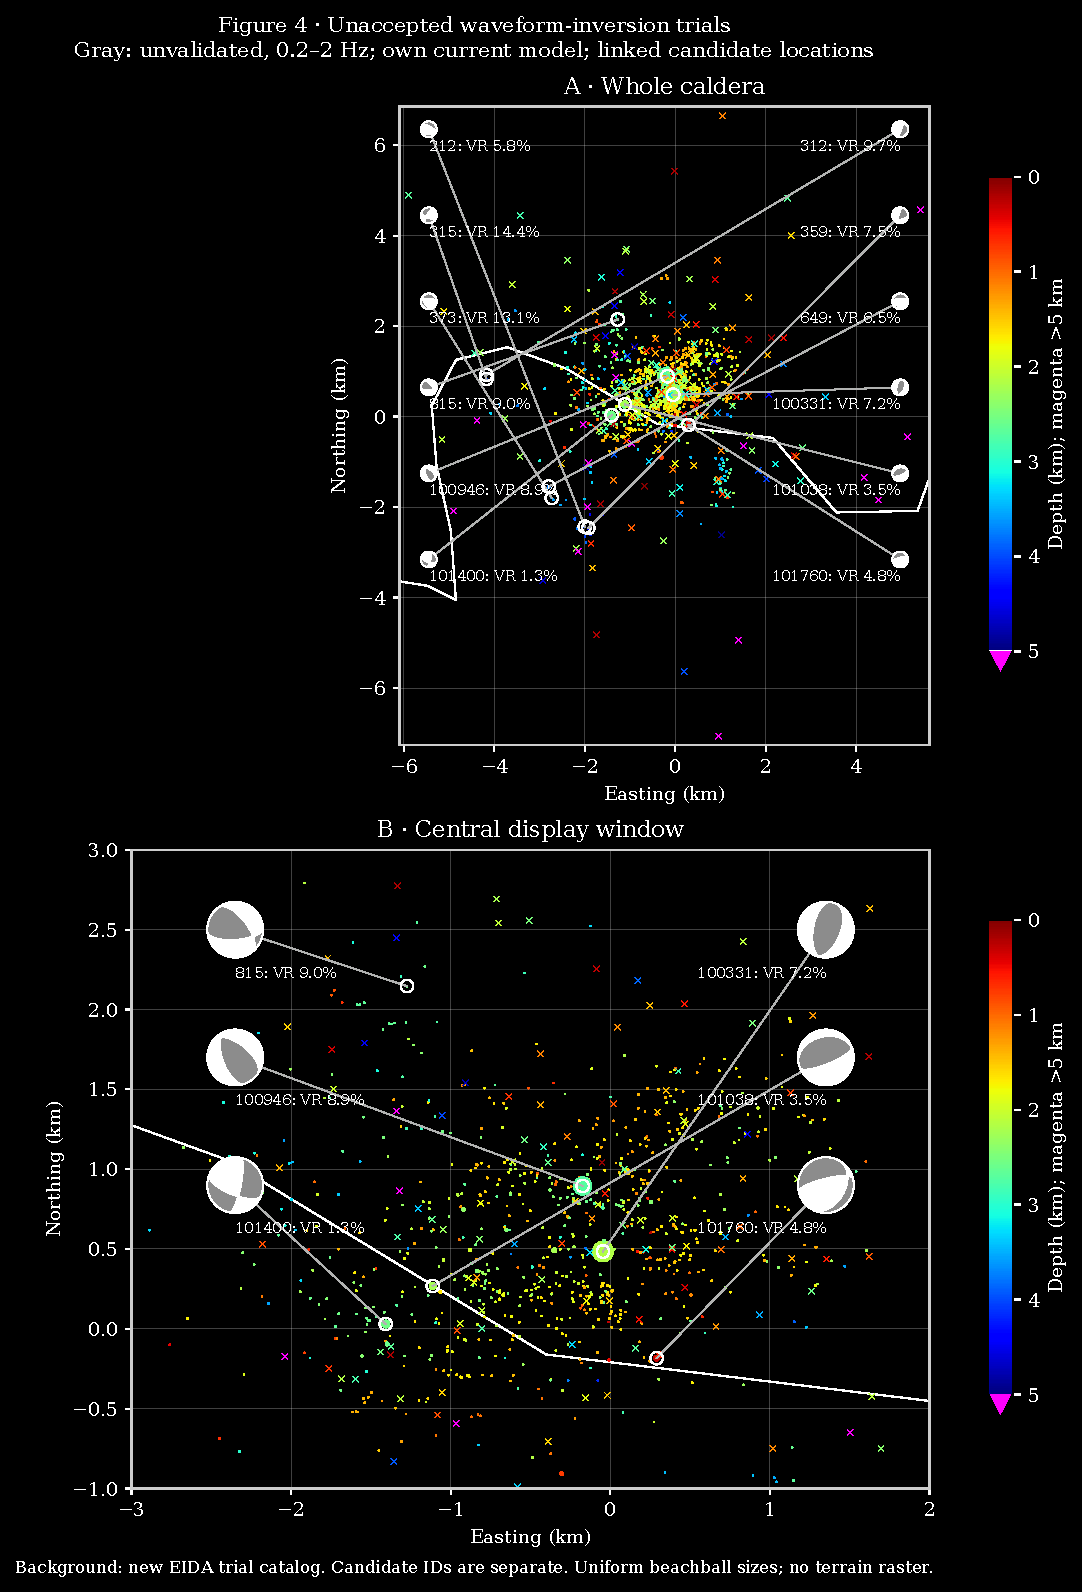
\includegraphics[width=.94\linewidth,height=0.620\textheight,keepaspectratio]{figures/figure_4_eida_followup.pdf}
\caption{Focal mechanisms of larger events. 12 unaccepted own FK/gCAP trial fits using newly available EIDA records and the current own model and explicitly linked own candidate geometry. 99 AI-reviewed polarities, 108 AI-reviewed ratios; no human review. SKHASH returns 2 solutions. Low-band variance reduction 1.3--14.4\%; orientations change 45.0--95.0 degrees between frequency bands. Gray beachballs denote unvalidated trials; background is the new independent catalog, never joined to candidates by integer ID. SKHASH returns 2 quality-D trials. No scientifically accepted mechanism. Partial/provisional: sparse observations, alternative association profile, unreviewed phases and unresolved model/location accuracy. Numerical generation is not agreement with the publication.}
\label{publication:4}
\end{figure}
